% Template for ICASSP-2010 paper; to be used with:
%          mlspconf.sty  - ICASSP/ICIP LaTeX style file adapted for MLSP, and
%          IEEEbib.bst - IEEE bibliography style file.
% --------------------------------------------------------------------------
\documentclass{article}
\usepackage{amsmath,graphicx,02456}
\usepackage{float}
\usepackage{appendix}

\toappear{02456 Deep Learning, DTU Compute, Fall 2021}

\def\x{{\mathbf x}}
\def\L{{\cal L}}

\title{Insect Classification Using Long Short-Term Memory}

\name{Freja Thoresen (S213769), Pascal Dufour (S011602), Nikolaj Sheller (C971666)\thanks{Thanks to FaunaPhotonics A/S for insect data.}}

\address{DTU \\ Department of Applied Mathematics and Computer Science}

\begin{document}

\maketitle

\begin{abstract}
The FaunaPhotonics insect sensor, can detect insects by observing near-infrared back-scattered light. 
The aim of this project is to classify signals as insects or not insects.
\end{abstract}
%
\begin{keywords}
insects, detection, non-destructive, unsupervised, near-infrared
\end{keywords}
%
\section{Introduction}
\label{sec:intro}

Automated, non-destructive insect detection in fields can improve pest control and spare beneficial insects in crops\cite{Kirkeby2021}.
The FaunaPhotonics insect sensor\cite{rydhmer2021automating}, the Volito, can detect insects by near-infrared (NIR) back-scatter.
The data provided by a Volito can be classified as insects, or not insects. 

The challenge is to do so reliably and quickly.

The Volito emits NIR and detects back-scatter using a charge-coupled device (CCD) sensor.
NIR back-scatters off an insect's carapace and wings as specular and diffuse reflections.
The reflections and wing beat frequency (WBF) produce a signature of the insect, that a deep neural network can be trained to identify and classify.
The CCD is sampled at $\sim$20KHz and produces a waveform when an insect traverses the probe volume, that is very similar to an audio signal a given insect produces, when flying. 
For a farmer to map insect prevalence in a field, the sensor must be mounted on a moving platform, e.g.\ a tractor or spraying boom.
When the sensor is in motion, significant noise is introduced in the acquired signal, e.g. from equipment vibration, crops traversing the probe volume etc.
The classification of insects need to be real-time such that the spraying boom can spray detected insects, while holding off in areas without activity.
This requires that our classification network be very robust to e.g.\ noise, rapid changes in baseline and vibration, while classifying real-time.


\section{Data preparation}

The raw data format of ten-minute data files with a sampling rate of 20 kHz\cite{rydhmer2021automating} provides a high resolution in the time dimension. However, the dimensional accuracy of the data provides a challenge when training the neural network; hence, the data were downsampled by ten. A honeybee has a wingbeat frequency of $234 \pm 13.9$ Hz\cite{10.1242/jeb.154609}; therefore, a sampling rate of 2000 is plentiful of a resolution to discover honeybees. 
For ten minutes, there are on average five honeybee flights in this experiment, giving a unbalance of the data since about $95 \:  \%$ will be labelled as not honeybees or negative, and about $5 \:  \%$ will be labelled as honeybees. After experimenting with weighting the loss function to adjust the unbalanced dataset, a better solution was to exclude more negative data points. The exclusion of negative data is as follows; if during 1000 data points, there has not been a divergence from the average of at least $10 \: \%$, exclude the period. In short, it will exclude periods in the data where there is mostly just a 'dead' signal. In order to have a tight window where the honeybee event is taking place, hence not including any flat signal, it was chosen to adjust the labelled data values, such that there needed at least a difference of 20 intensity in a window of 100 downsampled data points. 
The data can have different baselines, depending on the background light in the experiment, but the relative magnitude remains the same. Therefore, the data was normalized in ten-minute sequences to eliminate the baseline. 


\section{Results and Discussion}
After experimenting with different layers, such as LSTM and linear, it was found that a combination of a layered LSTM and a deep linear network provided the best results on different qualifiers. The evaluation was based on speed and quality since, given enough time, the networks would reach similar accuracies. MSE and Binary loss functions combined with an Adam optimizer provided similar results, albeit the combination of Binary loss and Adam was used since it is preferred for similar binary classification problems\cite{https://doi.org/10.1002/for.2585}. 


\subsection{Tuning of model}

The tuning was performed in two separate steps in order to minimize computational time. The first step was to tune learning rate and data formatting, and the second step was to tune neural network size and dropout rates. The full dataset was divided into training set ($80 \:  \%$), validation set ($10 \:  \%$), and test set ($10 \:  \%$).
The tuning of the learning rate and data formatting is in Figure \ref{fig:tune-data} and tuning of the neural network size and dropout rates are in Figure \ref{fig:tune-network}. The accuracies and loss were compared between the different hyperparameters. Furthermore, computational time was the final decider if two parameters were equally sufficient for the network quality. 

The threshold to determine if the output of the model is an insect was determined by the output values of the test set, which is in Figure \ref{fig:threshold}. The output values between 0 and 1 were well separated, and a threshold of 0.5 was used. 


\begin{figure*}[htb]
  \centering
  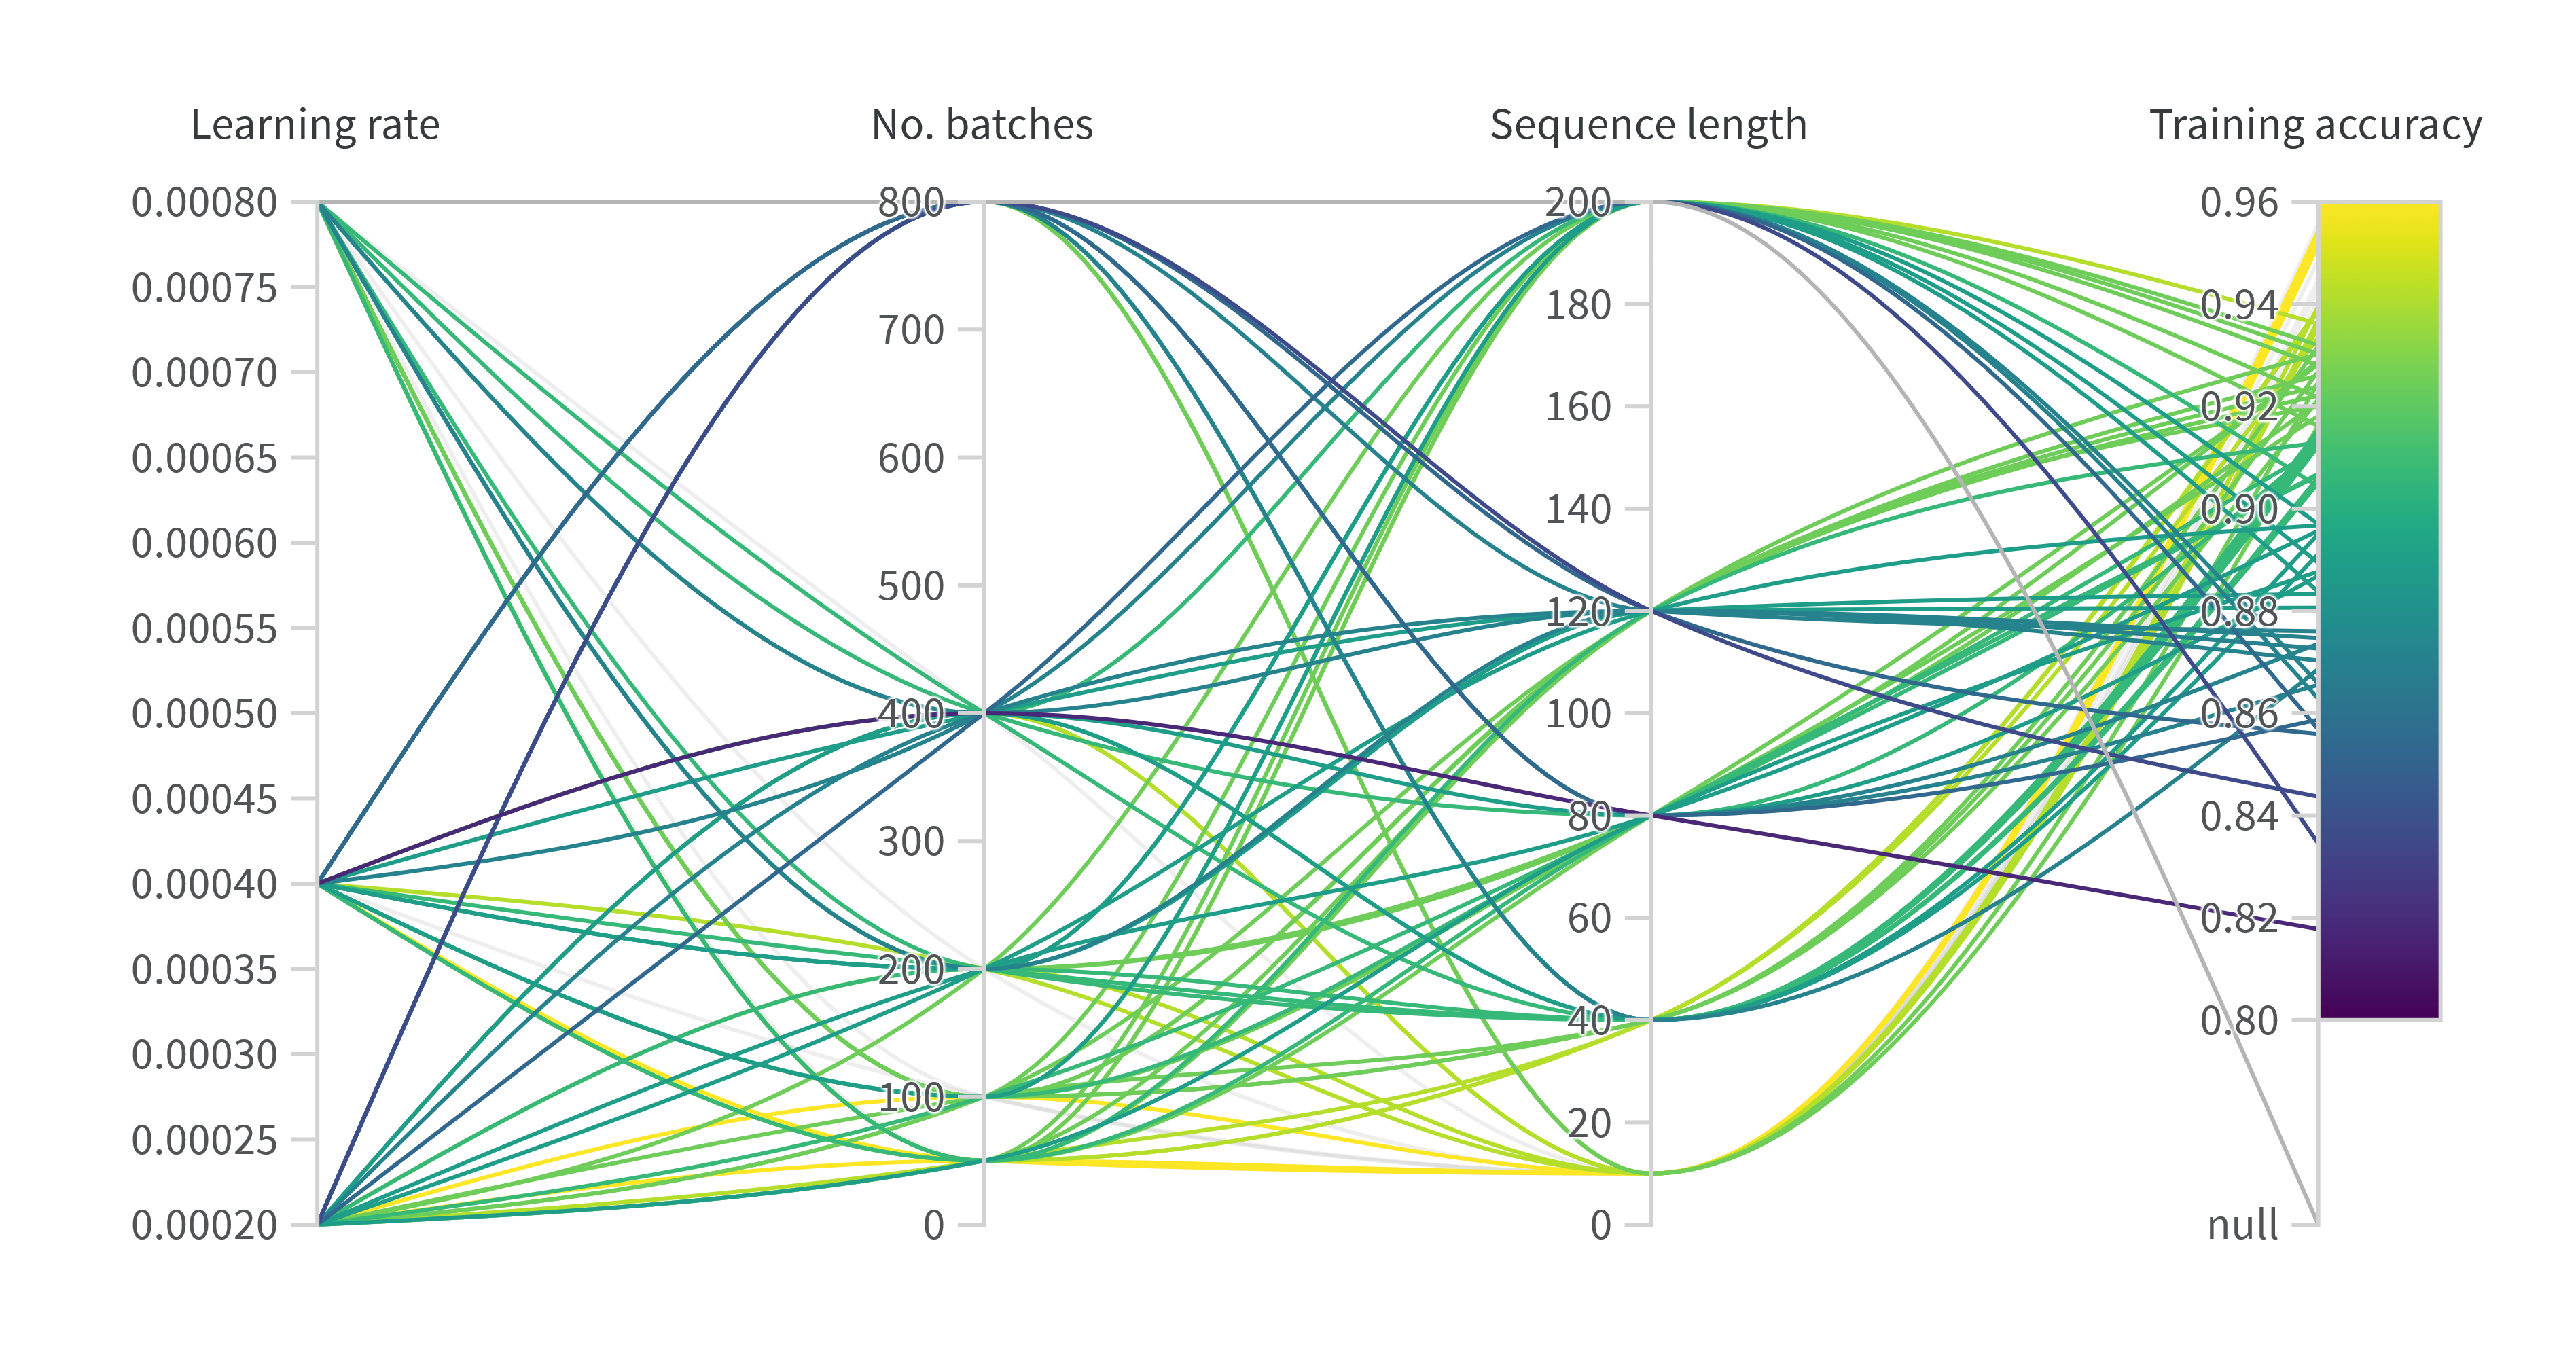
\includegraphics[width=0.8\textwidth]{Figures/data_tuning}
  \caption{Tuning of the learning rate and data parameters. There is a clear tendency that with a lower number of batches and lower sequence length, the training accuracy is high after 40 epochs. The best parameters were found to be a learning rate of 0.0002, 100 batches, and a sequence length of 10.}
  \label{fig:tune-data}
\end{figure*}

\begin{figure*}[htb]
  \centering
  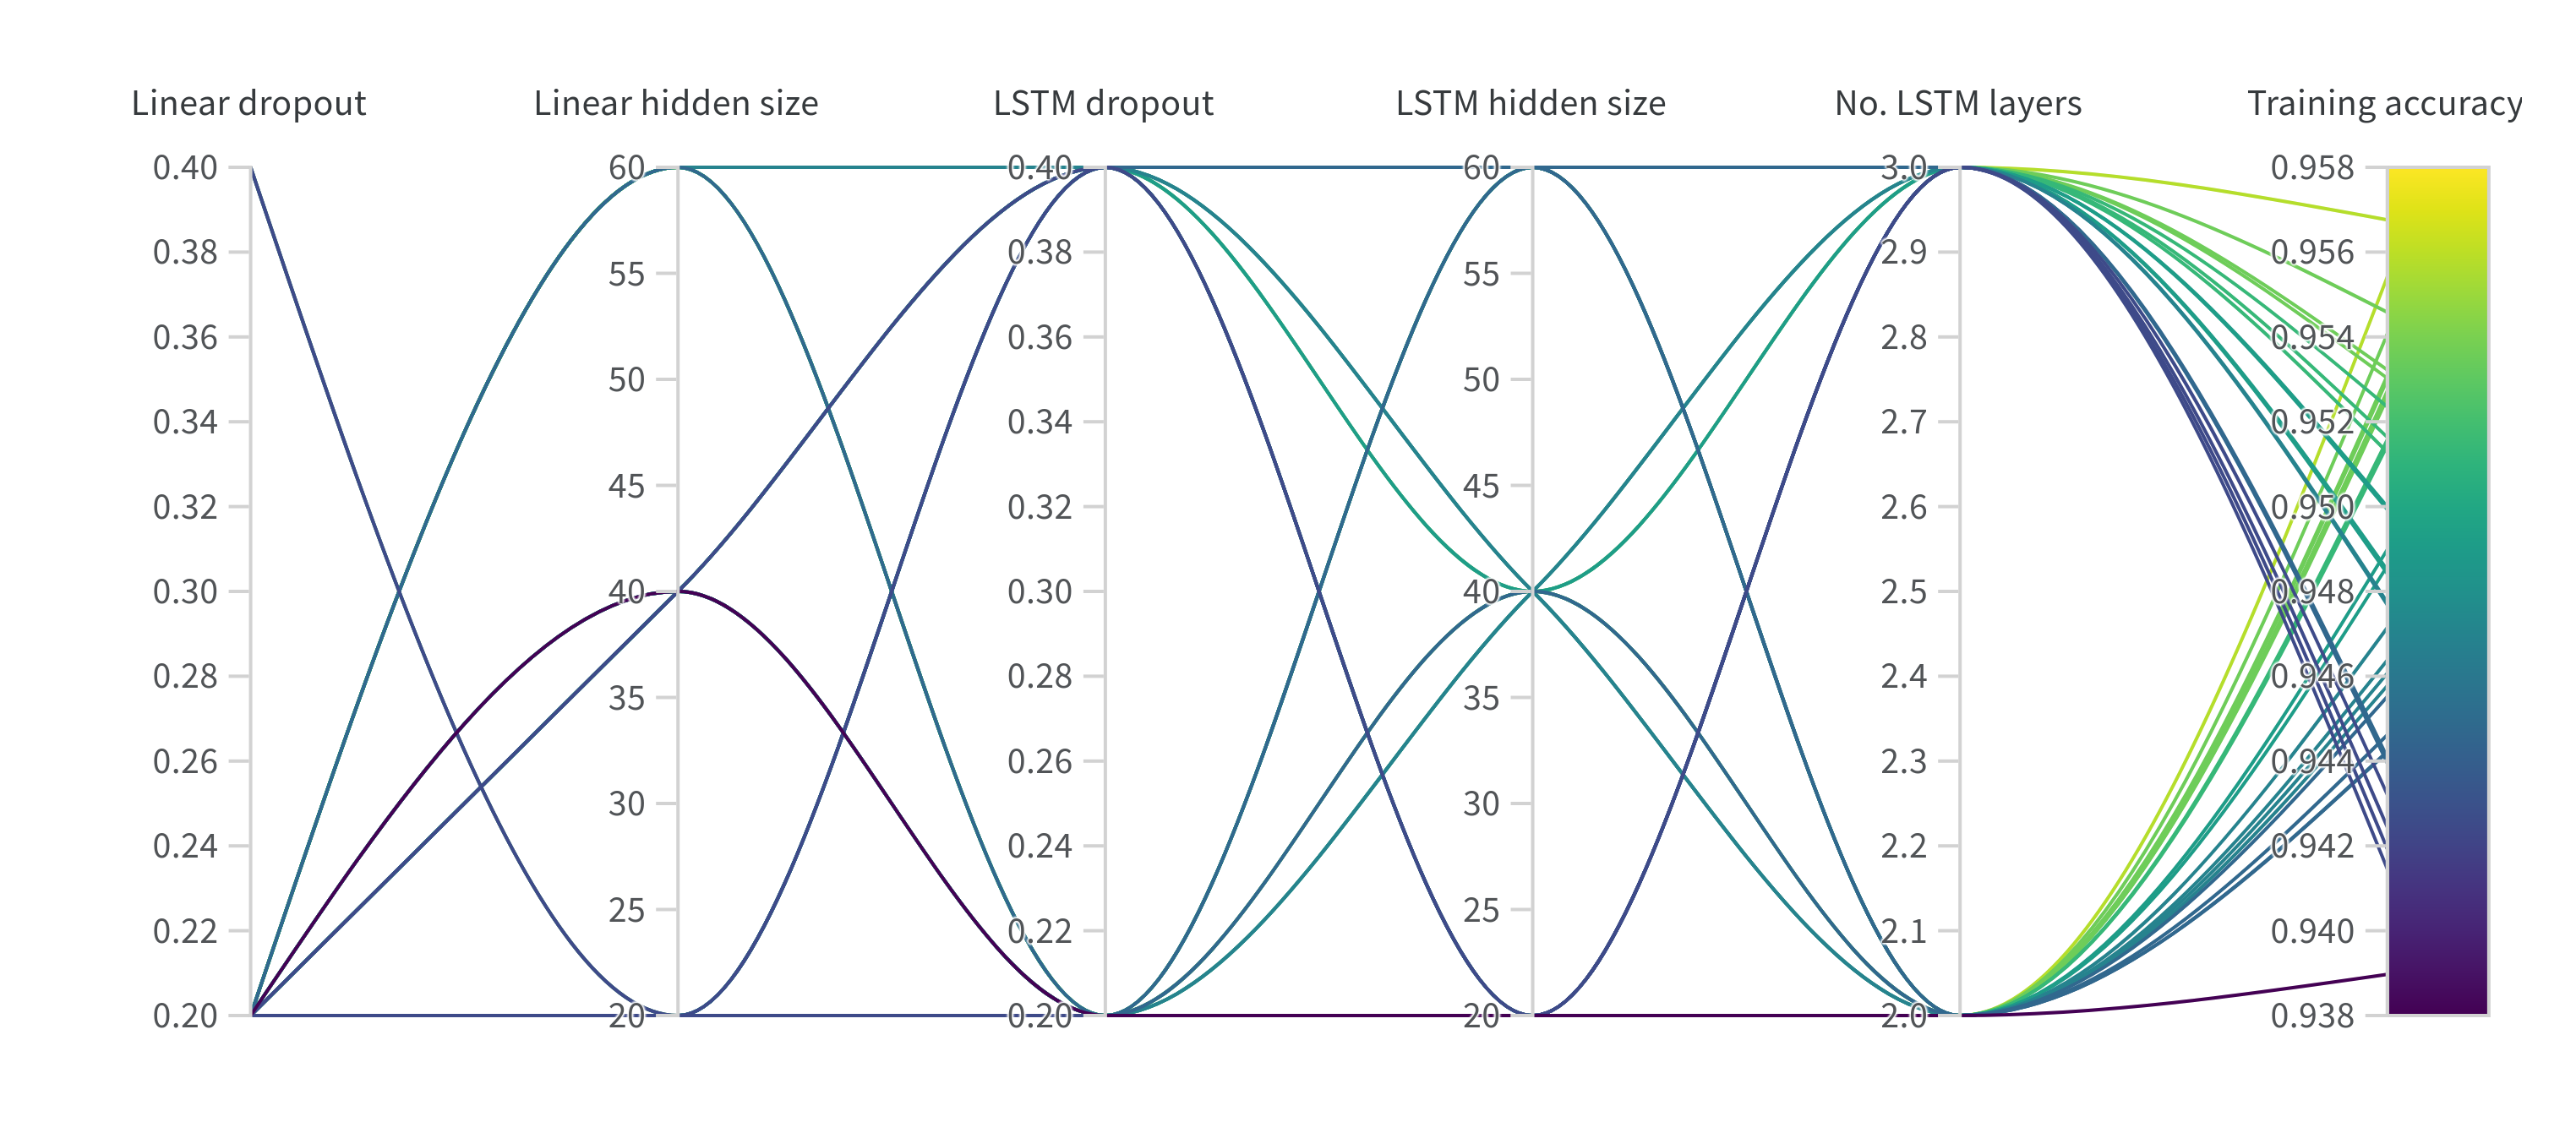
\includegraphics[width=\textwidth]{Figures/model_tuning}
  \caption{Tuning of the model parameters.}
  \label{fig:tune-network}
\end{figure*}

\begin{figure}[htb]
\begin{minipage}[b]{0.48\textwidth}
  \centering
  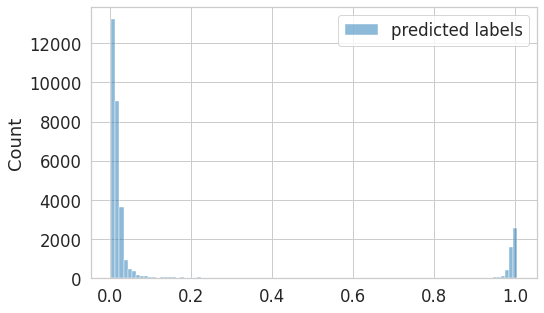
\includegraphics[width=6.0cm]{Figures/predicted_labels}
\end{minipage}
\caption{Predicted labels for the validation set. The values are very well seperated, and therefore a threshold of 0.5 is used to determine whether the predicted data is an insect.}
\label{fig:threshold}
\end{figure}

\subsection{Model results}
The accuracy and loss of the training and validation set are in Figure \ref{fig:acc_loss}. An early stopping with patience of 5 on the validation loss was used, meaning that if there is no improvement in the validation loss for 5 epochs, the training will end to prevent overfitting. The test dataset was used to find a model accuracy of $96.1 \: \%$. In Figure 5, an example of a prediction from the model is shown. In the right part of the figure, the model predicts the same as the labelled data. However, the model predicts an insect on the left side of the figure, where the labelled data does not. In this case, it is seen as a fault in the labelled data, and that the model can predict better than expected.


\begin{figure}[htb]
\begin{minipage}[b]{0.48\textwidth}
  \centering
  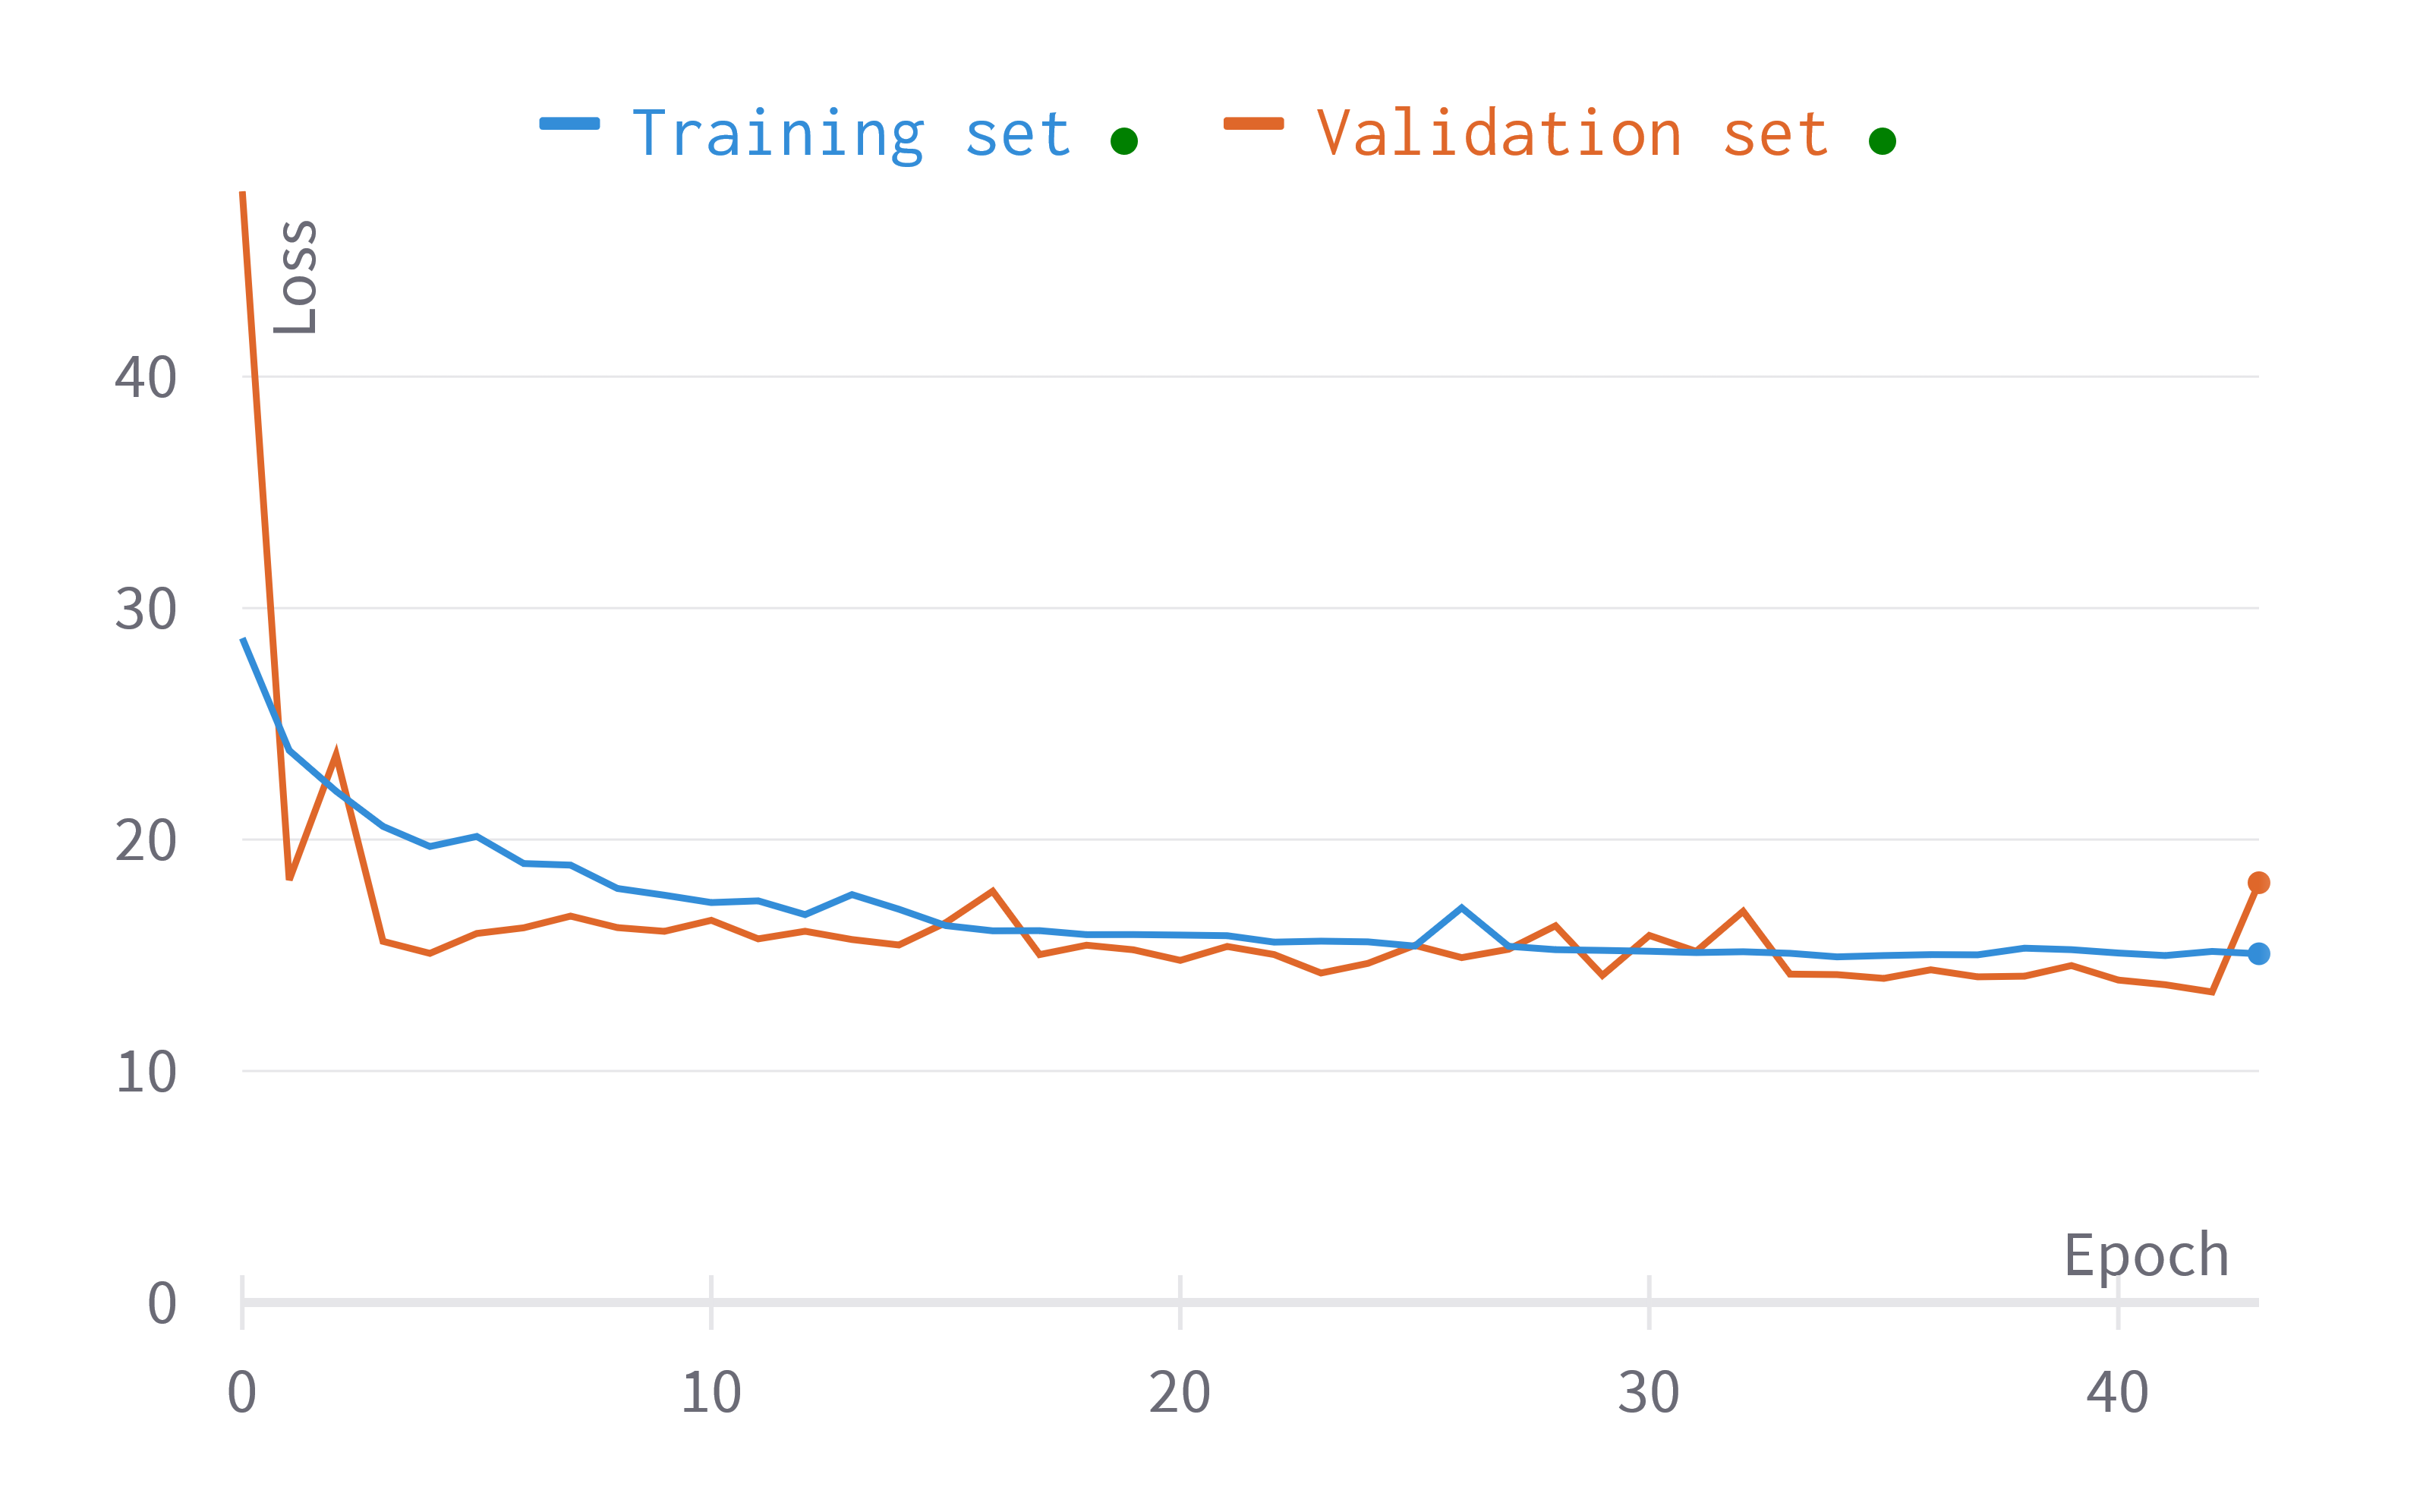
\includegraphics[width=7.5cm]{Figures/loss}
  \centerline{(a) Training and validation loss.}
\end{minipage}
\begin{minipage}[b]{.48\textwidth}
  \centering
  \centerline{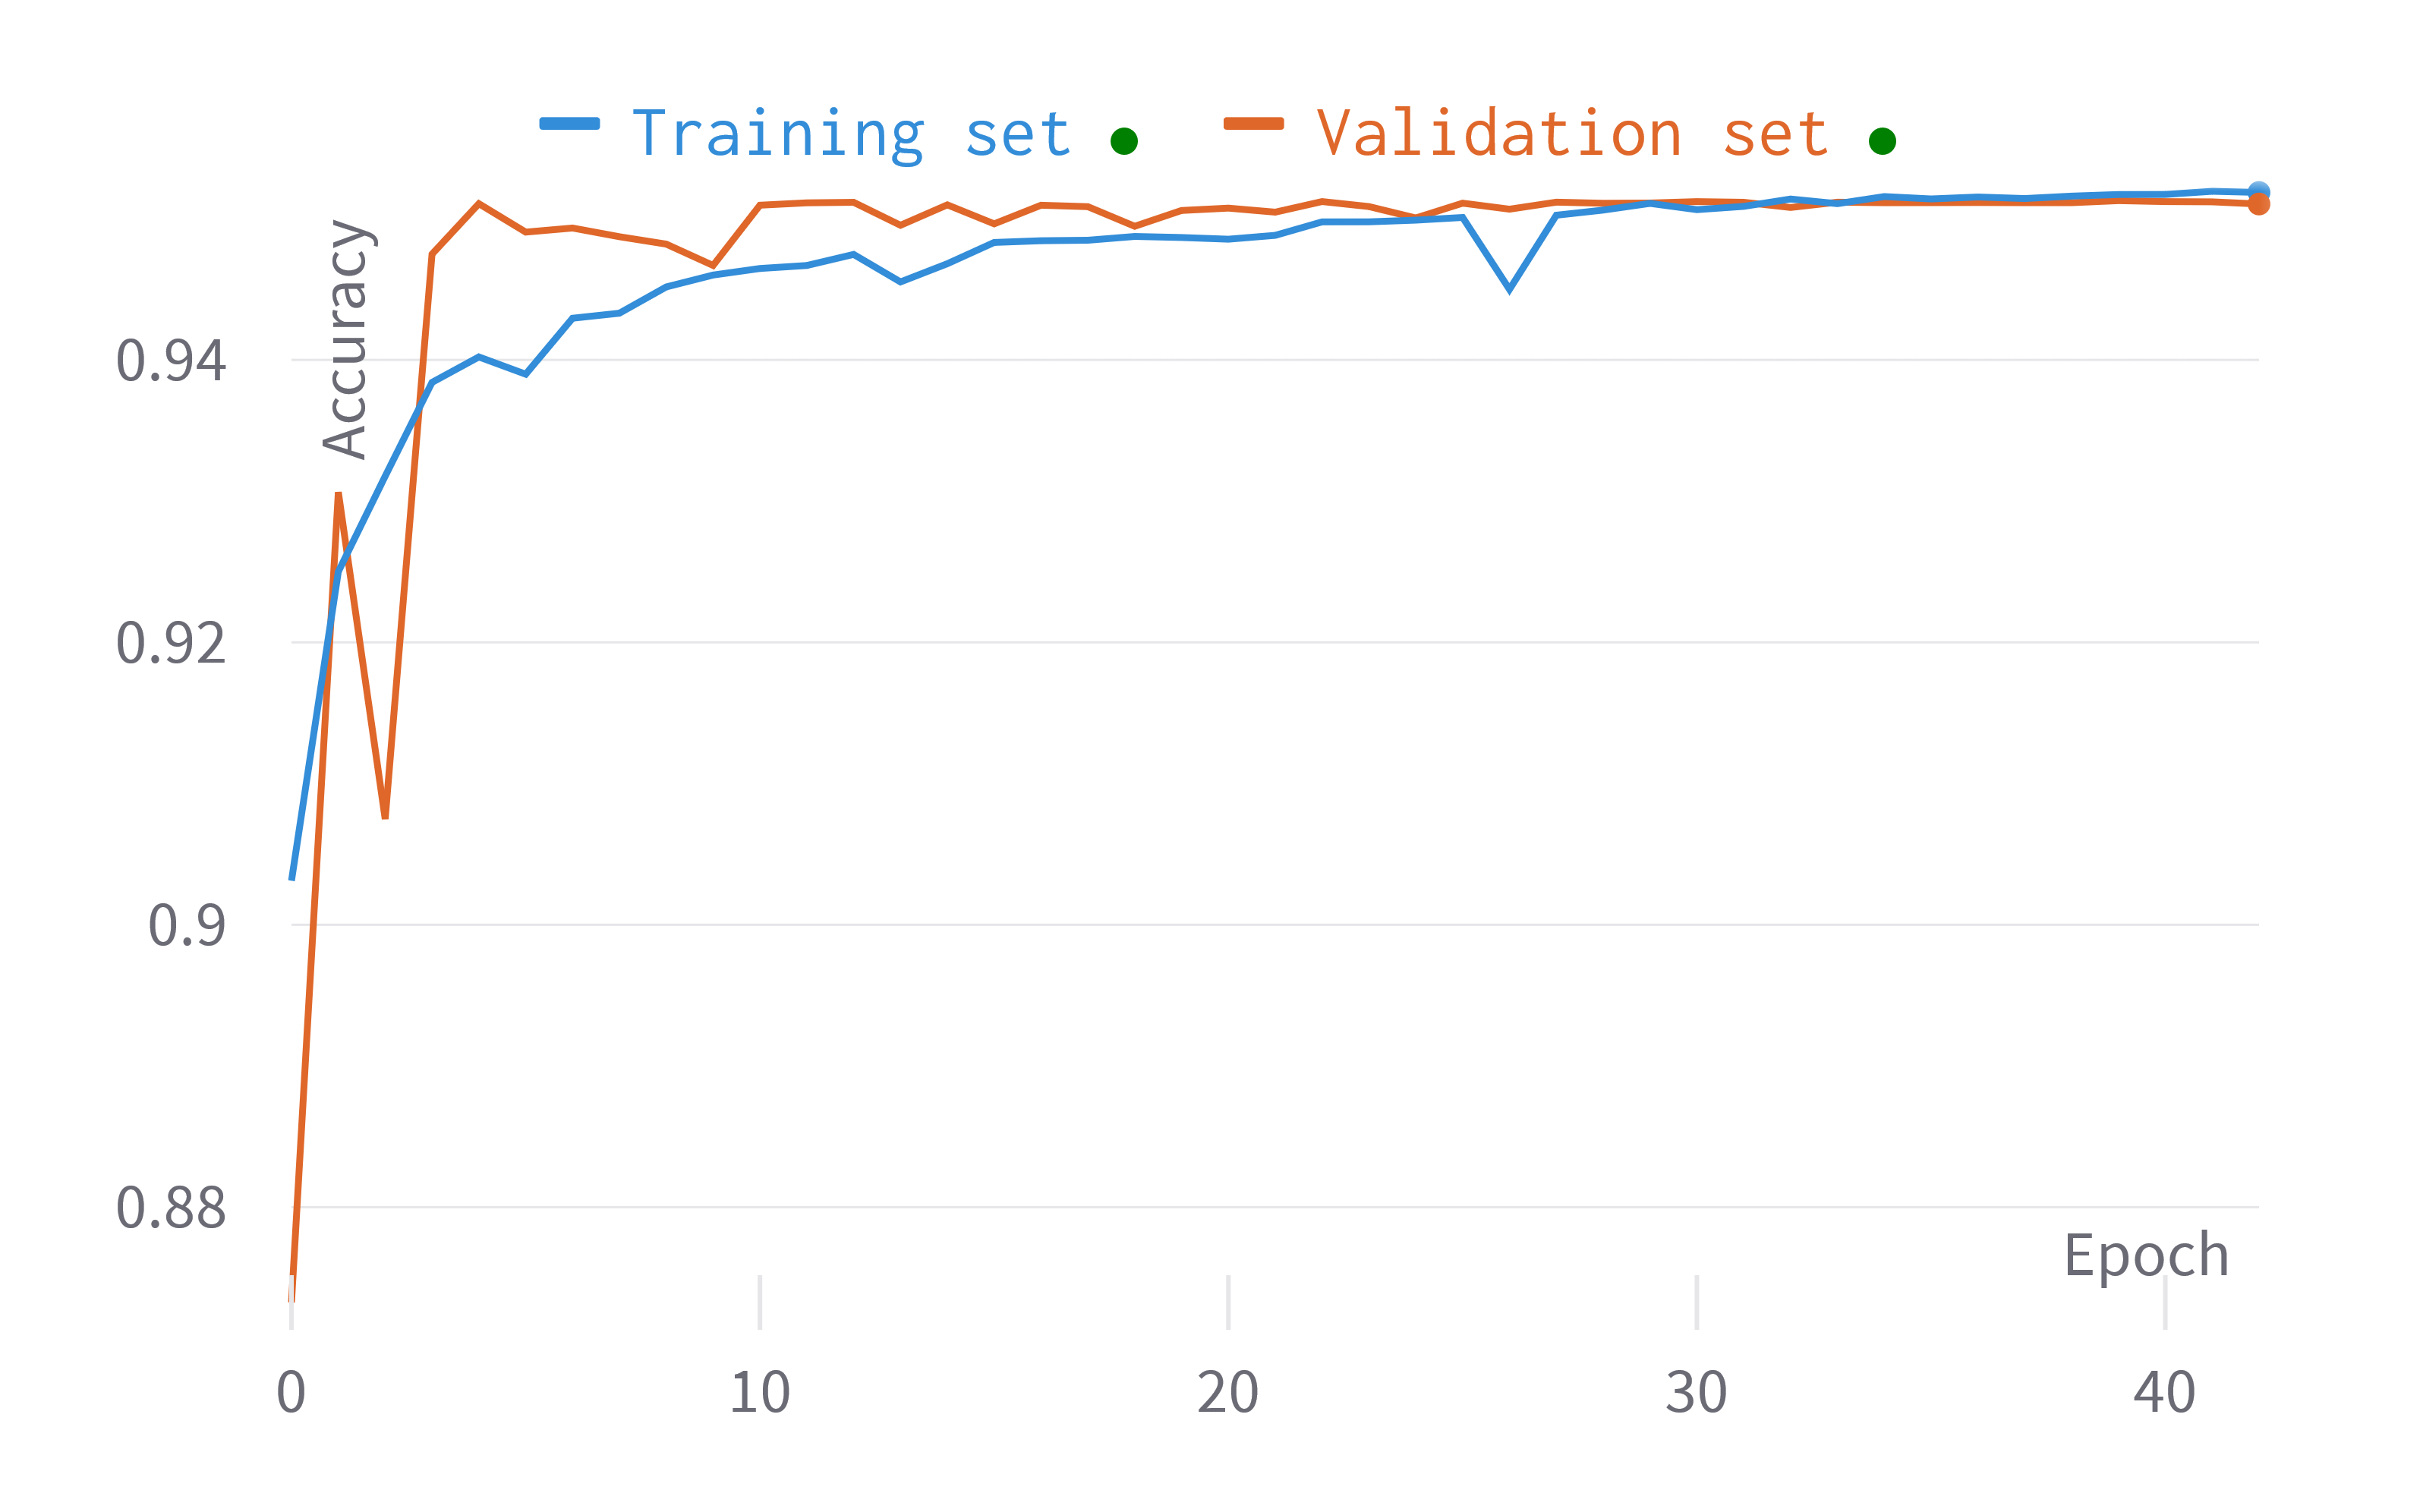
\includegraphics[width=7.5cm]{Figures/acc}}
  \centerline{(b) Training and validation accuracy}
\end{minipage}
\caption{Loss and accuracy for validation and training sets for the model.}
\label{fig:acc_loss}
\end{figure}

\begin{figure*}[htb]
  \centering
  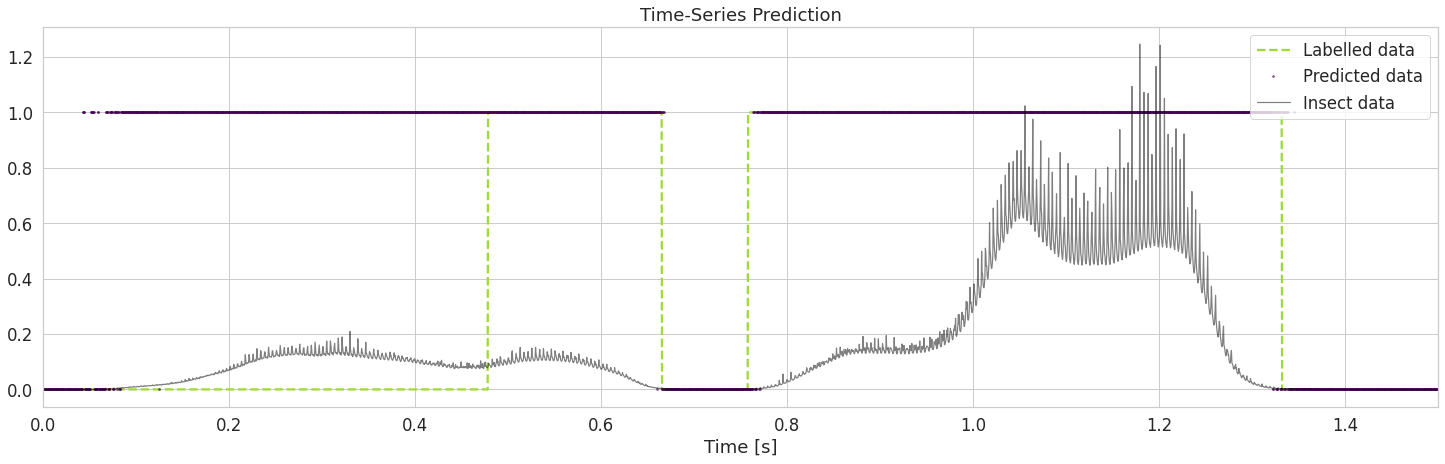
\includegraphics[width=\textwidth]{Figures/insect_results}
  \caption{Example of a model prediction. The striped line is the pre-labelled data, the line is the insect data, and the points are the model prediction. These cases were chosen to show one successful prediction (right) and another prediction (left). In the left-most prediction, where it is predicted as an insect, the labelled data states no insect. It looks like there is an insect to the human eye, even though the labelled data does not agree. This example was chosen to show that there has been an improvement in labelling the data as insect or not an insect, since the model prediction fits the data better.}
  \label{fig:predict}
\end{figure*}


\section{Conclusion}



% References should be produced using the bibtex program from suitable
% BiBTeX files (here: strings, refs, manuals). The IEEEbib.bst bibliography
% style file from IEEE produces unsorted bibliography list.
% -------------------------------------------------------------------------
\bibliographystyle{IEEEbib}
\bibliography{refs}

\end{document}
